\begin{savequote}[45mm]
\ascii{Any fool can write code that a computer can understand. Good programmers write code that humans can understand.}
\qauthor{\ascii{- Martin Flower}}
\end{savequote}

\chapter{线性模型} 
\label{ch:linear-model}

\section{逻辑回归}

\begin{content}

在逻辑回归(\ascii{Logistic Regression})中,$y$是一个实数值,且$y \in \{ 0,1\}$。但是,逻辑回归解决的是二分类问题。一般地,如果$y \ge 0.5$则判定为正类;否则判定为负类。

\[c = \left\{ \begin{gathered}
  1,y \ge 0.5 \hfill \\
  0,y < 0.5 \hfill \\ 
\end{gathered}  \right.\]

另外,常常使用\emph{指示函数}表达上式。

\[
c = \mathbb I(y \ge 0.5)
\]

其中,$\mathbb I(true) = 1$;否则$\mathbb I(false) = 0$。

\subsection{符号定义}

为了形式化地描述逻辑回归问题,此处定义了一些常用符号。需要注意的是,为了区分预测值与标签值的符号,因此使用$y, t$分别表示它们。

 \begin{itemize}
   \item \ascii{训练样本集}: $ S = \{ ({x^{(i)}},{t^{(i)}});i = 1,2,...,m\} $
   \item \ascii{第$i$个训练样本}: $ ({x^{(i)}},{t^{(i)}}) $
   \item \ascii{样本输入}: $ x = ({x_1},{x_2},...,{x_n})^{T}  \in {\mathbb{R}^n} $
   \item \ascii{样本标签}: $ t \in {\mathbb{R}} $
   \item \ascii{预测值}: $ y \in {\mathbb{R}} $   
   \item \ascii{误差值}: $ e = y - t \in {\mathbb{R}} $
   \item \ascii{权重}: $ w \in {\mathbb{R}^{n}} $   
   \item \ascii{偏置}: $ b \in {\mathbb{R}} $
   \item \ascii{线性加权和}: $ z = w^Tx + b \in {\mathbb{R}} $   
   \item \ascii{激活函数}: $ f(z) = \frac{1}{{1 + {e^{ - z}}}} \in {[0, 1]} $
   \item \ascii{正则项}: $ R(w) \in {\mathbb{R}} $
   \item \ascii{L2正则项}: $ \parallel w\parallel _2^2 \in {\mathbb{R}} $
   \item \ascii{损失函数(无正则项)}: $ L(w, b) \in {\mathbb{R}} $
   \item \ascii{损失函数(含正则项)}: $ J(w, b) = L(w, b) + \lambda R(w)\in {\mathbb{R}} $
   \item \ascii{梯度函数}: $ {\nabla _w}L( {w,b}) \in {\mathbb{R}^n} $
 \end{itemize}

\subsection{模型定义}

如\refig{logistic-regression-nn}所示,逻辑回归等价于仅具有一个神经元的网络模型。

\begin{figure}[H]
\centering
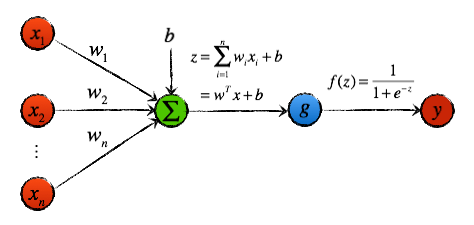
\includegraphics[width=0.6\textwidth]{figures/logistic-regression-nn.png}
\caption{逻辑回归:神经元模型}
 \label{fig:logistic-regression-nn}
\end{figure}

首先,逻辑回归完成$z = {w^T}x + b$的线性加权和;然后,使用\ascii{sigmoid}的激活函数,完成非线性变换。

\[\begin{aligned}
  y =  & {h_{w,b}}(x) \\ 
   =  & f({w^T}x + b) \\ 
   =  & \frac{1}{{1 + {e^{ - {w^T}x + b}}}} \\ 
\end{aligned} \]

$w$表示模型的权重,它是一个$n$维的向量;$b$表示神经元的偏置,它是一个标量。

\[\begin{gathered}
  w = \left[ {\begin{array}{*{20}{c}}
  {{w_1}} \\ 
  {{w_2}} \\ 
   \vdots  \\ 
  {{w_n}} 
\end{array}} \right] \in {\mathbb{R}^n} \\ 
  b \in \mathbb{R} \\ 
\end{gathered} \]

$x$表示模型的输入,它是一个$n$维的向量;其中,$\forall {x_i} \in x,i = 1,2,...,n$,它表示输入向量$x$的一个特征值;$y$表示模型的输出,它是一个标量。

\[\begin{gathered}
  x = \left[ {\begin{array}{*{20}{c}}
  {{x_1}} \\ 
  {{x_2}} \\ 
   \vdots  \\ 
  {{x_n}} 
\end{array}} \right] \in {\mathbb{R}^n} \\ 
  {\text{y}} \in {\mathbb{R}} \\ 
\end{gathered}\]

$f(z)$是神经元的激活函数,此处使用\ascii{sigmoid}函数。

\subsection{Sigmoid函数}

\ascii{sigmoid}函数将无穷的定义域空间压缩为$[0, 1]$的值域空间,因此具有天然的概率解释意义。

\[
f(z) = \frac{1}{{1 + {e^{ - z}}}}
\]


\subsubsection{软饱和性}

如\refig{sigmoid}所示,\ascii{sigmoid}函数具有软饱和性,即

\[\begin{gathered}
  \mathop {\lim }\limits_{z \to  + \infty } f(z) = 1 \hfill \\
  \mathop {\lim }\limits_{z \to  - \infty } f(z) = 0 \hfill \\ 
\end{gathered} \]

\begin{figure}[H]
\centering
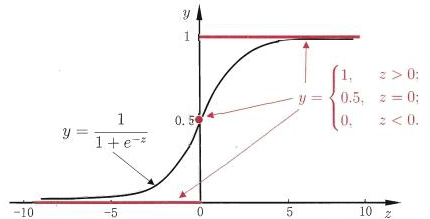
\includegraphics[width=0.6\textwidth]{figures/sigmoid.png}
\caption{sigmoid函数}
 \label{fig:sigmoid}
\end{figure}

\subsubsection{导数}

\ascii{sigmoid}的导数具有特殊的表现形式,其导函数是$y$的二次函数。令

\[
y = \frac{1}{{1 + {e^{ - z}}}}
\]

根据链式求导法则,可以很容易地推导出\ascii{sigmoid}的导数。

\[\begin{aligned}
  y' =  & \frac{d}{{dz}}\left( {\frac{1}{{1 + {e^{ - z}}}}} \right) \\ 
   =  & \frac{d}{{dz}}{\left( {1 + {e^{ - z}}} \right)^{ - 1}} \\ 
   =  &  - {\left( {1 + {e^{ - z}}} \right)^{ - 2}}\frac{d}{{dz}}\left( {{e^{ - z}}} \right) \\ 
   =  &  - {\left( {1 + {e^{ - z}}} \right)^{ - 2}}{e^{ - z}}\frac{d}{{dz}}\left( { - z} \right) \\ 
   =  &  - {\left( {1 + {e^{ - z}}} \right)^{ - 2}}{e^{ - z}}\left( { - 1} \right) \\ 
   =  & \frac{{{e^{ - z}}}}{{{{\left( {1 + {e^{ - z}}} \right)}^2}}} \\ 
   =  & \frac{1}{{1 + {e^{ - z}}}}\left( {1 - \frac{1}{{1 + {e^{ - z}}}}} \right) \\ 
   =  & y(1 - y) \\ 
\end{aligned} \]

\subsection{概率解释}

对于任意的$(x,t) \in S$,根据\ascii{Sigmoid}的函数特性,假设$t|x$服从$Bernoulli(y)$的概率分布。

\[\begin{aligned}
  P(t = 1|x;w,b) = & y \\ 
  P(t = 0|x;w,b) = & 1 - y \\ 
\end{aligned} \]

众所周知,$Bernoulli(y)$概率分布可以描述为如下更为简洁的表达方式。

\[P(t|x;w,b) = {y^t}{(1 - y)^{1 - t}}\]

推而广之,假如存在$m$个独立同分布的训练样本$\{ ({x^{(i)}},{t^{(i)}});i = 1,2,...,m\}$,以$(w,b)$为参数的似然函数可表达为:

\[\begin{aligned}
  L(w,b) =  & P\left( {\vec y|X} \right) \\ 
   =  & \prod\limits_{i = 1}^m {P\left( {{t^{(i)}}|{x^{(i)}};w,b} \right)}  \\ 
   =  & \prod\limits_{i = 1}^m {{{\left( {{y^{(i)}}} \right)}^{{t^{(i)}}}}{{\left( {1 - {y^{(i)}}} \right)}^{1 - {t^{(i)}}}}}  \\ 
\end{aligned} \]

其中,
${y^{(i)}} = {h_{w,b}}({x^{(i)}}), i=1,2,...,m $。一般地,根据对数函数的单调递增性,将其变换为对数似然函数,使得连乘运算转换为连加运算,简化了问题的复杂度。

\[l(w,b) = \log L(w,b) = \sum\limits_{i = 1}^m {{t^{(i)}}\log {y^{(i)}} + \left( {1 - {t^{(i)}}} \right)\log \left( {1 - {y^{(i)}}} \right)} \]

因此,逻辑回归问题可以转换为最大化对数似然函数的参数估计问题。

\[\hat w,\hat b = \arg \mathop {\max }\limits_{w,b} \sum\limits_{i = 1}^m {{t^{(i)}}\log {y^{(i)}} + \left( {1 - {t^{(i)}}} \right)\log \left( {1 - {y^{(i)}}} \right)} \]

可以使用梯度上升的优化方法,迭代求取最优的参数$(\hat w,\hat b)$。

\subsection{交叉熵损失函数}

在机器学习领域中,常常使用\emph{损失函数},并使用\emph{梯度下降}的优化算法,迭代求取最优的参数$(\hat w,\hat b)$。根据上一节的推导,给定一个训练样本$(x, t)$,逻辑回归可以使用如下定义的损失函数,它是交叉熵损失函数在二分类问题下的特殊表现形式。

\[L(w,b;x,t) =  - \left\{ {t\log y + \left( {1 - t} \right)\log \left( {1 - y} \right)} \right\}\]

推而广之,给定训练数据集$ S = \{ ({x^{(i)}},{t^{(i)}});i = 1,2,...,m\} $,逻辑回归的损失函数可以表达为:

\[L(w,b; S) =  - \sum\limits_{i = 1}^m {{t^{(i)}}\log {y^{(i)}} + \left( {1 - {t^{(i)}}} \right)\log \left( {1 - {y^{(i)}}} \right)} \]

因此,逻辑回归的学习问题便转换为最小化损失函数$L(w,b)$的优化问题。

\[\hat w,\hat b = \arg \mathop {\min }\limits_{w,b} L(w, b)\]

\subsection{正则项}

为了控制模型的复杂度,可以增加$L2$的正则项,它等于向量$w$的内积。

\[R(w) = \lambda \parallel w\parallel _2^2 = {w^T}w \]

其中,$\lambda$称为正则项因子,用于控制正则项的影响程度;它是模型的超参数,可以通过交叉验证试验获取最佳的数值。增加了正则项后,模型的损失函数可以表达为:

\[J(w,b) = L(w,b) + \lambda \parallel w\parallel _2^2\]

其优化问题也随之表达为:

\[\hat w,\hat b = \arg \mathop {\min }\limits_{w,b} J(w, b)\]

\subsection{梯度下降}

可以使用梯度下降算法,迭代求取最优的$(\hat w,\hat b)$。其中,$\alpha$表示学习速率,表示参数更新的大小。

\[\begin{aligned}
  w \leftarrow & w - \alpha {\nabla _w}L(w,b) \\ 
  b \leftarrow & b - \alpha {\nabla _b}L(w,b) \\ 
\end{aligned} \]

其中,$w,b$的梯度分别定义为:

\[\begin{aligned}
  {\nabla _w}L(w,b) = & \frac{{\partial L}}{{\partial w}} \\ 
  {\nabla _b}L(w,b) = & \frac{{\partial L}}{{\partial b}} \\ 
\end{aligned} \]

如\refig{mnist-gd}所示,可以将损失函数比作一座山,登山者试图寻找最佳的行动方案达到山谷。登山者站在某个山坡上环顾四周,决定沿梯度的反方向向下走一小步,直到获得更优的解。当实施梯度下降更新算法时,初始点不同,获得的最小值可能也不同。因此梯度下降求得的只是局部最小值。

\begin{figure}[H]
\centering
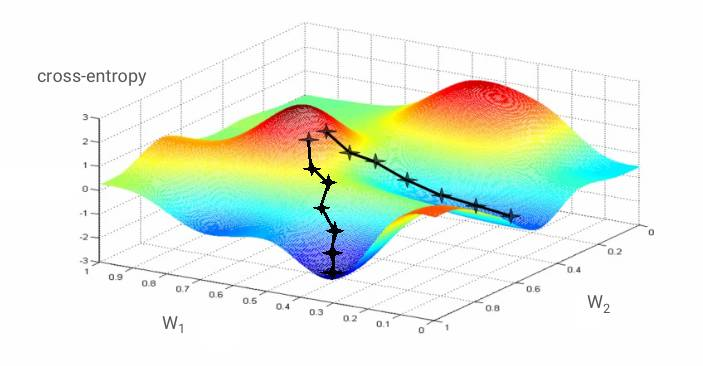
\includegraphics[width=0.8\textwidth]{figures/mnist-gd.jpeg}
\caption{梯度下降算法}
 \label{fig:mnist-gd}
\end{figure}

梯度下降的步伐大小非常重要,如果太小,则找到函数最小值的速度就很慢;如果太大,则可能会越过极值点。一般地,在模型训练初期,因为离模型收敛的目标还比较远,因此将其学习速率调得大一些;随着迭代次数增加,学习速率调得小一些。因此,学习速率$\alpha$是自适应的,目前理论上存在很多学习速率$\alpha$随时间衰减的优化算法,例如\ascii{Adagrad}等。因此,优化问题的关键在于梯度如何计算。

\subsection{计算梯度}

根据链式求导法则,给定任意一个样本$ (x,t) \in S $,可以推导出$ L(y, t) $相对于$ w_i, i=1,2,...,n $的梯度公式。

\[\begin{aligned}
  \frac{{\partial L}}{{\partial {w_i}}}
   =  & \frac{{\partial L}}{{\partial y}}\frac{{\partial y}}{{\partial z}}\frac{{\partial z}}{{\partial {w_i}}} \\ 
   =  & \left( {\frac{{1 - t}}{{1 - y}} - \frac{t}{y}} \right)y(1 - y){x_i} \\ 
   =  & (y - t){x_i} \\ 
\end{aligned} \]

同理,可以推导出$ L(W,b) $相对于$ b $的梯度公式。

\[\begin{aligned}
  \frac{{\partial L}}{{\partial b}} 
   =  & \frac{{\partial L}}{{\partial y}}\frac{{\partial y}}{{\partial z}}\frac{{\partial z}}{{\partial b}} \\ 
   =  & \left( {\frac{{1 - t}}{{1 - y}} - \frac{t}{y}} \right)y(1 - y) \\ 
   =  & y - t \\ 
\end{aligned} \]

进一步,通过矢量化得到$w,b$的梯度计算公式。其中,$\nabla _w}L( {w,b;x,t}) \in {\mathbb{R}^{n}}$,$\nabla _b}L( {w,b;x,t}) \in {\mathbb{R}}$。

\[\begin{gathered}
  {\nabla _w}L( {w,b;x,t}) =  \left({y - t} \right)x \\ 
  {\nabla _b}L( {w,b;x,t) =   y - t  \\ 
\end{gathered} \]

推而广之,给定训练数据集$ S = \{ ({x^{(i)}},{t^{(i)}});i = 1,2,...,m\} $,得到$w,b$的矢量化的梯度计算公式为:

\[\begin{gathered}
  {\nabla _w}L(w,b;S) = \left( {\frac{1}{m}\sum\limits_{i = 1}^m {\left( {{y^{(i)}} - {t^{(i)}}} \right)} } \right)x \\ 
  {\nabla _b}L(w,b;S) = \frac{1}{m}\sum\limits_{i = 1}^m {\left( {{y^{(i)}} - {t^{(i)}}} \right)}  \\ 
\end{gathered} \]

\subsection{参数更新}

参数更新存在三种基本的算法。对于给定一个训练样本$ ({x^{(i)}},{t^{(i)}}) $,根据$w, b$的梯度公式,完成本次迭代的参数更新,该算法常称为\emph{随机梯度下降法}(\ascii{SGD})。因为更新一次参数,\ascii{SGD}只需读取一个训练样本,而单个样本并不能代表普遍性,可能存在很多噪声,因此模型的收敛情况较为抖动。但是,\ascii{SGD}可以实现模型的快速收敛,效率较为高效。

\[\begin{gathered}
  w \leftarrow w - \alpha \left( {{y^{(i)}} - {t^{(i)}}} \right)x \\ 
  b \leftarrow b - \alpha \left( {{y^{(i)}} - {t^{(i)}}} \right) \\ 
\end{gathered} \]

另外一种极端,给定整个训练样本数据$ S $,根据$w, b$的梯度公式,完成本次迭代的参数更新,该算法常称为\emph{批式梯度下降法}(\ascii{BGD})。因为更新一次参数,需要遍历整个训练数据集,因此模型收敛较为平稳。但是,由于计算量大,模型收敛速度相对\ascii{SGD}较为缓慢。

\[\begin{gathered}
  w \leftarrow w - \alpha \left( {\frac{1}{m}\sum\limits_{i = 1}^m {\left( {{y^{(i)}} - {t^{(i)}}} \right)} } \right)x \\ 
  b \leftarrow b - \alpha \left( {\frac{1}{m}\sum\limits_{i = 1}^m {\left( {{y^{(i)}} - {t^{(i)}}} \right)} } \right) \\ 
\end{gathered} \]

而在现实应用中,既不会使用\ascii{BGD},也不会使用\ascii{SGD},而使用\ascii{MiniBatch}的\ascii{SGD}算法。更为甚者,由于\ascii{MiniBatch}的\ascii{SGD}的大规模应用,因此常简称\ascii{MiniBatch}的\ascii{SGD}为\ascii{SGD}算法。

\[\begin{aligned}
  w \leftarrow w - \alpha \left( {\frac{1}{{batch\_zie}}\sum\limits_{i = 1}^{batch\_size} {\left( {{y^{(i)}} - {t^{(i)}}} \right)} } \right)x \\ 
  b \leftarrow b - \alpha \left( {\frac{1}{{batch\_size}}\sum\limits_{i = 1}^{batch\_size} {\left( {{y^{(i)}} - {t^{(i)}}} \right)} } \right) \\ 
\end{aligned} \]

相对于\ascii{BGD},\ascii{MiniBatch}的\ascii{SGD}每次跟新参数不用遍历真个训练数据集,只需遍历一个\ascii{batch\_size}个训练样本;因此,相对\ascii{BGD},\ascii{MiniBatch}的\ascii{SGD}的收敛速度更快。而相对于\ascii{SGD},\ascii{MiniBatch}的\ascii{SGD}每次跟新参数,读取携带更多普遍性的\ascii{batch\_size}个训练样本;因此,相对\ascii{SGD},\ascii{MiniBatch}的\ascii{SGD}的收敛更为平稳。

\subsection{计算图}

一般地,当使用神经网络表示学习模型时,其训练过程都包括两个基本步骤:

\begin{itemize}
  \item \ascii{正向计算}: 计算损失
  \item \ascii{反向传播}: 计算梯度
\end{itemize}

为了实现正向的损失计算,及其反向的梯度计算,可以将网络翻译为等价的计算图。在正向的计算图中,节点描述了某种抽象的数学运算,例如矩阵乘法,向量内积,激活函数等;边表示函数的输出值,并作为下游节点函数的输入。



如\refig{logistic-bp}所示,逻辑回归的正向

\begin{figure}[H]
\centering
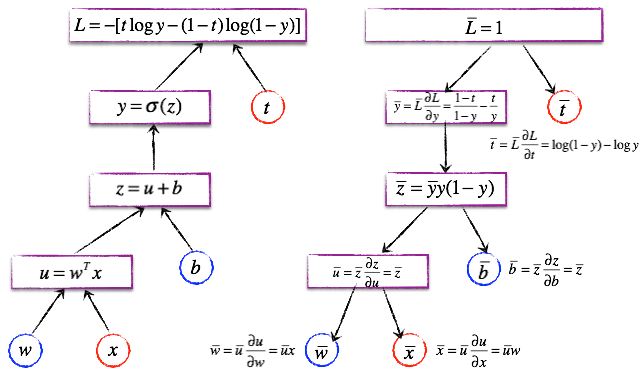
\includegraphics[width=0.8\textwidth]{figures/logistic-bp.png}
\caption{逻辑回归:前向计算与反向传播}
 \label{fig:logistic-bp}
\end{figure}


\end{content}

\section{单层感知器}

\begin{content}

首先,尝试构建\ascii{10}个神经元的单层感知器。如\refig{mnist-slp}所示,对于诸如手写数字识别的多分类问题,理论上常使用\ascii{softmax}的激活函数。

\begin{figure}[H]
\centering
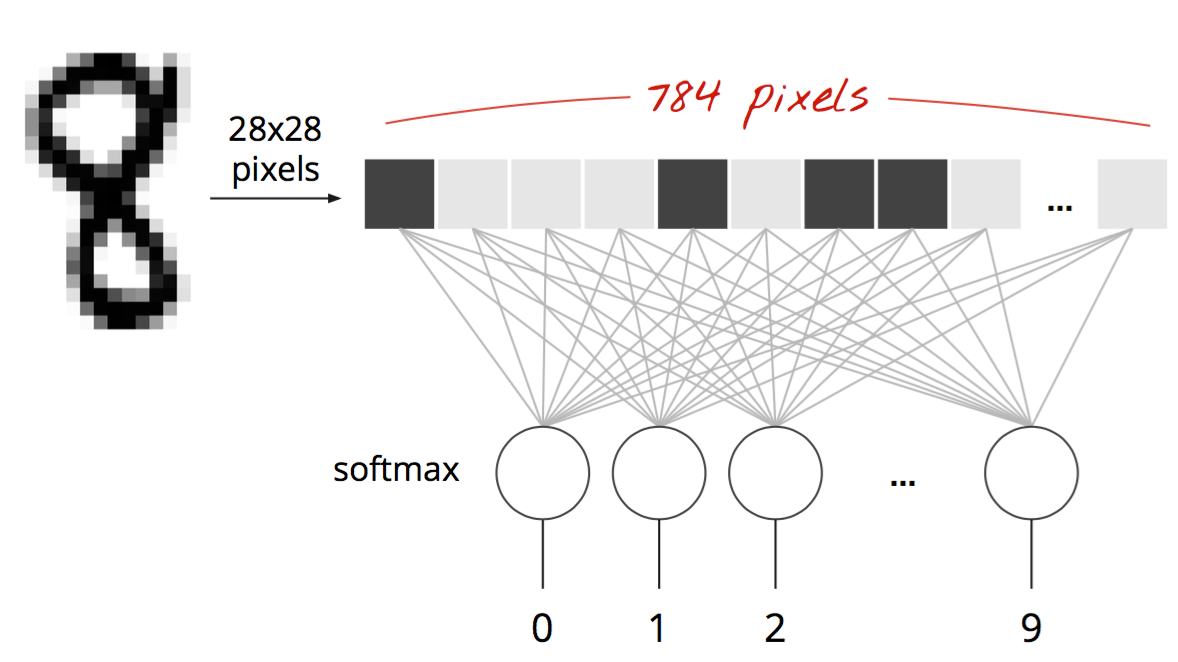
\includegraphics[width=0.8\textwidth]{figures/mnist-slp.png}
\caption{单层感知器}
 \label{fig:mnist-slp}
\end{figure}

\subsection{理论基础}

理论上,\ascii{softmax}回归是\ascii{logistic}回归的广义扩展。其中,\ascii{logistic}回归是为了解决二分类问题,即$y \in \{ 0,1\}$;而\ascii{softmax}回归是为了解决$ k $分类问题,即$y \in \{ 1,2,...,k\}$。

\subsubsection{符号定义}

为了形式化地描述\ascii{softmax}回归问题,此处定义了一些常用符号。

 \begin{itemize}
   \item \ascii{训练样本集}: $ S = \{ ({x^{(i)}},{y^{(i)}});i = 1,2,...,m\} $
   \item \ascii{第$i$个训练样本}: $ ({x^{(i)}},{y^{(i)}}) $
   \item \ascii{样本输入}: $ x = ({x_1},{x_2},...,{x_n})^{T}  \in {\mathbb{R}^n} $
   \item \ascii{样本标签(one-hot)}: $ y = ({y_1},{y_2},...,{y_k})^{T} \in {\mathbb{R}^k} $
   \item \ascii{权重}: $ W \in {\mathbb{R}^{n \times k}} $   
   \item \ascii{偏置}: $ b \in {\mathbb{R}^k} $   
   \item \ascii{softmax函数}: $ 
softmax {(z_i)} = \tfrac{{{e^{{z_i}}}}}{{\sum\limits_{j = 1}^k {{e^{{z_j}}}} }}  \quad i = 1,2,...,k
$
 \end{itemize}

\subsubsection{softmax函数}

如\refig{softmax}所示,模型先求取线性加权和$z$,然后求取$e^z$,最后再实施归一化操作。

\begin{figure}[H]
\centering
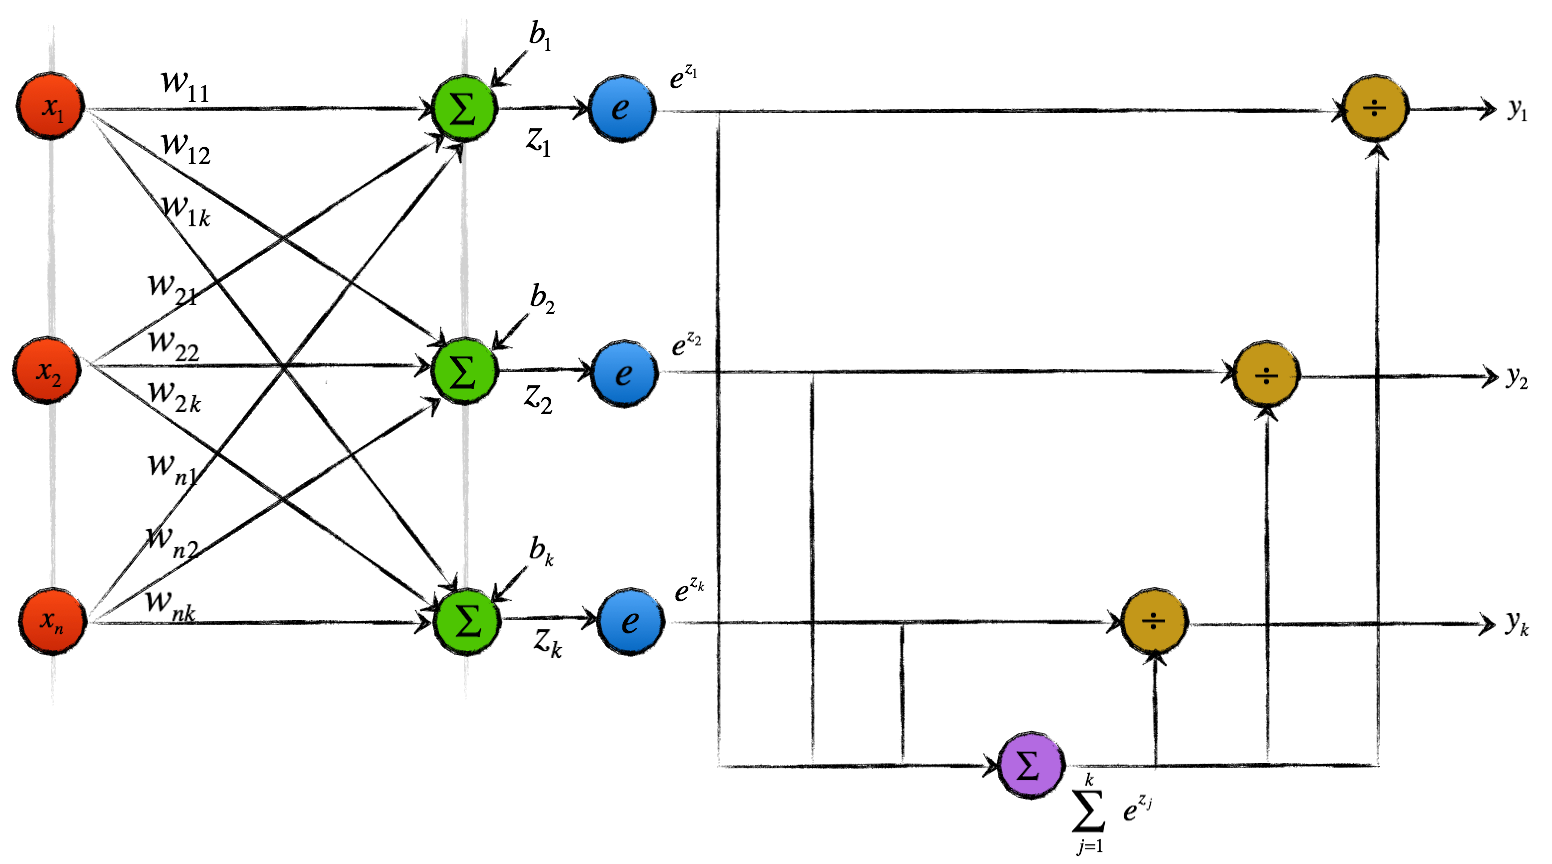
\includegraphics[width=0.8\textwidth]{figures/softmax.png}
\caption{softmax函数}
 \label{fig:softmax}
\end{figure}

\subsubsection{权重与偏置}

权重$W$为一个$n \times k$的二维矩阵。

\[
W = \left( {{W_1},{W_2},...,{W_k}} \right) = \left( {\begin{array}{*{20}{c}}
  {{w_{11}}}& \ldots &{{w_{1k}}} \\ 
   \vdots & \ddots & \vdots  \\ 
  {{w_{n1}}}& \cdots &{{w_{nk}}} 
\end{array}} \right) \in {\mathbb{R}^{n \times k}}
\]

其中,$W_j$是一个长度为$n$的向量。

\[
{W_j} = {\left( {{w_{1j}},{w_{2j}},...,{w_{nj}}} \right)^T} \in {\mathbb{R}^n}, j = 1,2,...,k \\
\]

而偏置$b$是一个长度为$k$的\ascii{\quo{one-hot}}向量。

\[
b = {({b_1},{b_2},...,{b_k})^T} \in {\mathbb{R}^k}
\]

\subsubsection{模型定义}

多分类问题的单层感知器模型,使用\ascii{softmax}激活函数,可以如此定义。

\[\begin{aligned}
  y =  & {h_{W,b}}(x) = softmax (z) = softmax ({W^T}x + b) \\ 
   =  & {\left( {{y_1},{y_2},...,{y_k}} \right)^T} \\ 
   =  & \frac{1}{{\sum\limits_{j = 1}^k {{e^{{z_j}}}} }}{\left( {{e^{{z_1}}},{e^{{z_2}}},...,{e^{{z_k}}}} \right)^T} \\ 
   =  & \frac{1}{{\sum\limits_{j = 1}^k {{e^{W_j^Tx + {b_j}}}} }}{\left( {{e^{W_1^Tx + {b_1}}},{e^{W_2^Tx + {b_2}}},...,{e^{W_k^Tx + {b_k}}}} \right)^T} \ 
\end{aligned} \]

其中,对于任意给定的样本$ (x, y) \in S $,$ z_i $表示$W_i^Tx+b_i$的线性加权和,而$y_i(i=1,2,...,k)$表示将其划归为类$i$的概率。

\[\begin{gathered}
  P\left( {y = i|x;W,b} \right) = \frac{{{e^{W_i^Tx + b_i}}}}{{\sum\limits_{j = 1}^k {{e^{W_j^Tx + b_j}}} }} \hfill \\
  i = 1,2,...,k \hfill \\ 
\end{gathered} \]


\subsubsection{交叉熵函数}

基于样本数据集$ S = \{ ({x^{(i)}},{y^{(i)}});i = 1,2,...,m\} $,交叉熵损失函数可以如此定义。

\[\begin{aligned}
  J(W,b) =  &  - \frac{1}{m}\sum\limits_{i = 1}^m {{y^{(i)}}\log \left( {{{\widehat y}^{(i)}}} \right)}  \\ 
   =  &  - \frac{1}{m}\sum\limits_{i = 1}^m {\sum\limits_{j = 1}^k {y_j^{(i)}\log \left( {\widehat y_j^{(i)}} \right)} }  \\
\end{aligned} \]

\ascii{softmax}多分类问题,就是求取最优解$(W^*,b^*)$,使得

\[W^*,b^* = \mathop {\arg \min }\limits_{W,b} J(W,b)\]

\subsubsection{计算梯度}

对于任意一个样本$ (x,y) \in S $,可以推导出$ J(W,b) $相对于$ W $与$ b $的梯度公式。

\[\begin{aligned}
  {\nabla _W}J\left( {W,b;x,y} \right) =  & \left( {\widehat y - y} \right)x \\ 
  {\nabla _b}J\left( {W,b;{x^{(i)}},{y^{(i)}}} \right) =  & \left( {\widehat y - y} \right) \\ 
\end{aligned} \]


\subsubsection{参数更新}

对于训练样本数据$ S $,根据$W, b$的梯度公式,完成本次迭代的参数更新。

\[\begin{aligned}
  W \leftarrow  & W - \alpha \frac{{\sum\limits_{i = 1}^m {{\nabla _W}J\left( {W,b;{x^{(i)}},{y^{(i)}}} \right)} }}{m} \\ 
  b \leftarrow  & b - \alpha \frac{{\sum\limits_{i = 1}^m {{\nabla _b}J\left( {W,b;{x^{(i)}},{y^{(i)}}} \right)} }}{m} \\ 
\end{aligned} \]

\subsection{定义模型}

接下来,使用\tf{}完成该模型的搭建和训练。需要注意的是,理论上的公式与\tf{}具体实现存在微妙的差异。理论上,公式中的$x$常表示一个样本,但\tf{}中的\code{x}常表示一个\ascii{mini-batch}的样本数据集。因此,使用\tf{}设计网络模型时,需要特别关注各个张量大小的变化是否符合预期。

\subsubsection{输入和标签}

首先,使用\code{tf.placeholder}分别定义训练样本的输入和标签。

\begin{leftbar}
\begin{python}
x = tf.placeholder(tf.float32, [None, 28, 28, 1])
t = tf.placeholder(tf.float32, [None, 10])
\end{python}
\end{leftbar}

\code{tf.placeholder}定义了一个占位的\ascii{OP}。\code{None}表示未确定的样本数目,此处表示\code{batch\_size}的大小;当\code{Session.run}时,将通过\code{feed\_dict}的字典提供一个\ascii{mini-batch}的样本数据集,从而自动推导出\code{tf.placeholder}的大小。

另外,每张图片使用$ 28 \times 28 \times 1 $的三维数据表示(灰度为\ascii{1})。为了简化问题,此处将输入的样本数据扁平化,将其变换为长度为\ascii{784}的一维向量。其中,\ascii{-1}表示\ascii{mini-batch}的样本数目,由运行时自动推演其大小。

\begin{leftbar}
\begin{python}
x = tf.reshape(x, [-1, 784])
\end{python}
\end{leftbar}

\subsubsection{定义变量}

然后,使用\code{tf.Variable}定义模型参数。定义训练参数时,必须指定参数的初始化值;训练参数将根据初始值,自动推演数据的类型,及其大小。

\begin{leftbar}
\begin{python}
w = tf.Variable(tf.zeros([784, 10]))
b = tf.Variable(tf.zeros([10]))
\end{python}
\end{leftbar}

此外,变量在使用之前,必须完成初始化。此处,\code{init\_op}将初始化所有全局的训练参数。

\begin{leftbar}
\begin{python}
init_op = tf.global_variables_initializer()
\end{python}
\end{leftbar}

\subsubsection{模型定义}

接下来,便可以很容易地得到多分类问题的单层感知器模型。

\begin{leftbar}
\begin{python}
y = tf.nn.softmax(tf.matmul(x, w) + b)
\end{python}
\end{leftbar}

如\refig{mnist-linear-sum}所示,首先计算\code{x}与\code{w}的矩阵乘法,让后将\code{b}广播(\ascii{broadcast})到矩阵的每一行相加,最终得到训练参数的线性加权和。

\begin{figure}[H]
\centering
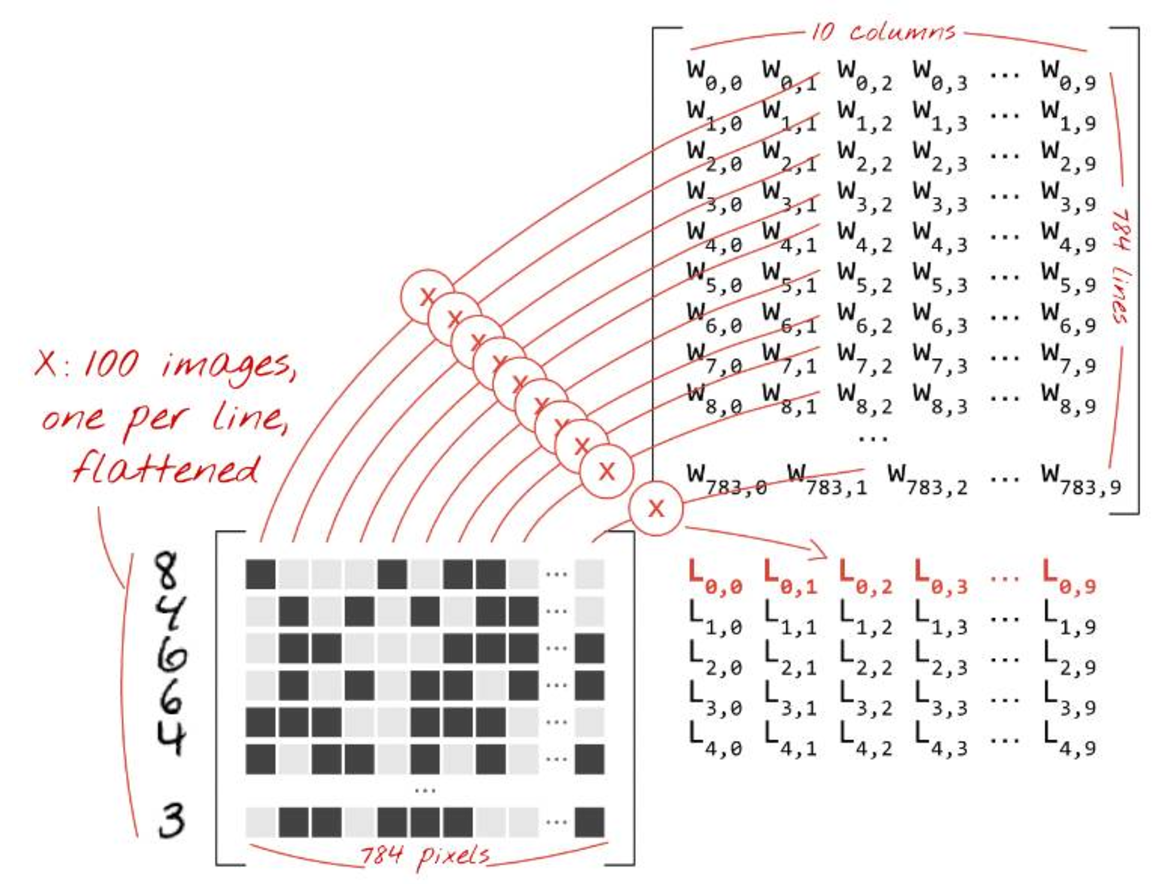
\includegraphics[width=0.8\textwidth]{figures/mnist-linear-sum.png}
\caption{线性加权和}
 \label{fig:mnist-linear-sum}
\end{figure}

如\refig{mnist-softmax}所示,\ascii{softmax}将逐行实施运算,最终,\code{y}的大小为\code{[100, 10]}。

\begin{figure}[H]
\centering
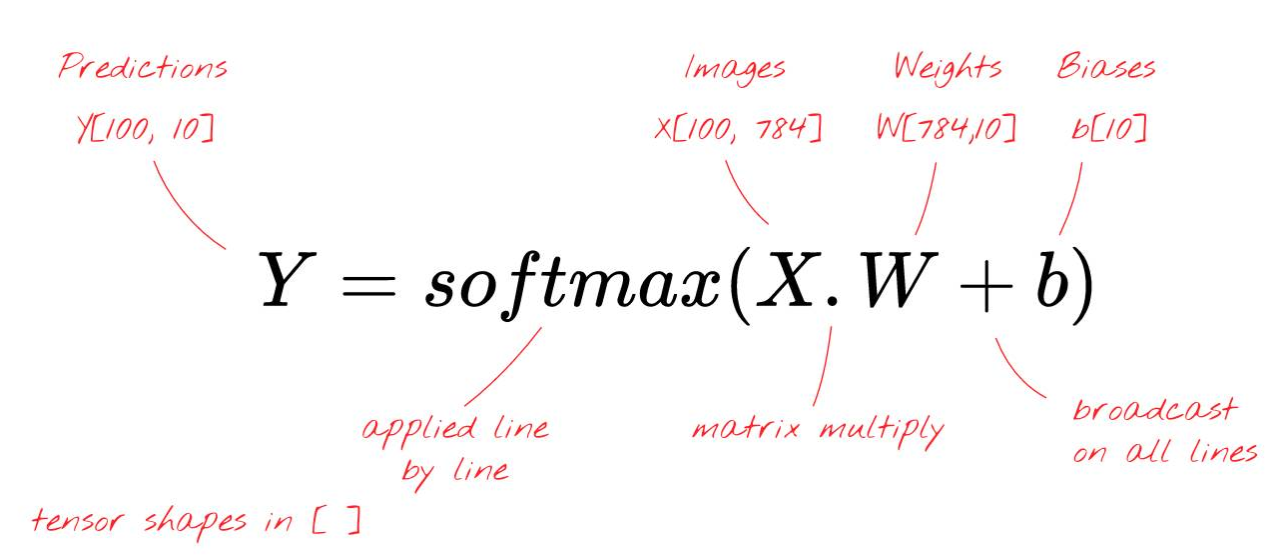
\includegraphics[width=0.8\textwidth]{figures/mnist-softmax.png}
\caption{激活函数:softmax}
 \label{fig:mnist-softmax}
\end{figure}

\subsubsection{损失函数}

对于多分类问题,可以使用交叉熵的损失函数。

\begin{leftbar}
\begin{python}
cross_entropy = -tf.reduce_sum(t * tf.log(y))
\end{python}
\end{leftbar}

如\refig{mnist-cross-entropy}所示,\code{t}和\code{y}的大小都为\code{[100, 10]};特殊地,\code{t}的每一行都是一个\quo{\ascii{one-hot}}向量。

对\code{y}实施\code{tf.log}操作,也将得到一个大小为\code{[100, 10]}的矩阵。然后,\code{t}与\code{tf.log(y)}逐位相乘(并非矩阵相乘),也将得到大小为\code{[100, 10]}的矩阵。最终,\code{tf.reduce\_sum}将矩阵中所有元素相加,得到一个标量(\ascii{scalar})值。

\begin{figure}[H]
\centering
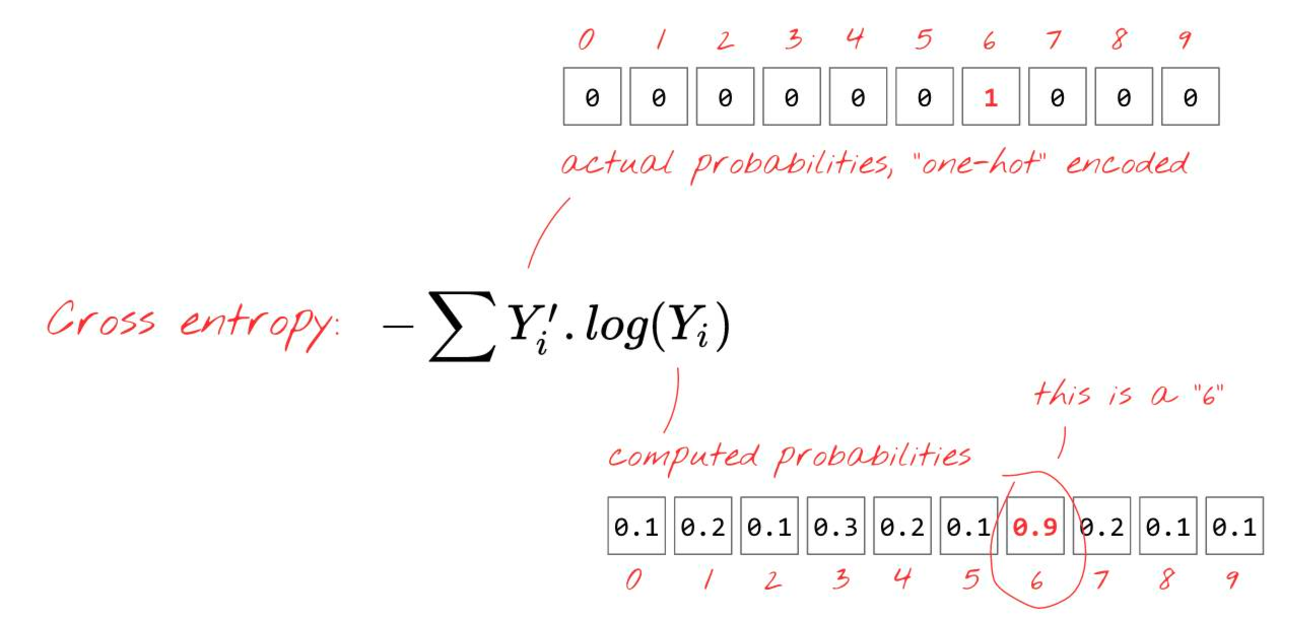
\includegraphics[width=0.8\textwidth]{figures/mnist-cross-entropy.png}
\caption{交叉熵损失函数}
 \label{fig:mnist-cross-entropy}
\end{figure}

\subsubsection{精度}

\code{tf.argmax(y,1)}将按第\ascii{1}个维度计算最大值的索引。既按照$ y_{100 \times 10} $的每一行,计算得到在每一行中最大值的的索引值。因此,\code{tf.argmax(y,1)}将得到大小为\code{[100, 1]}的矩阵,或大小为\ascii{100}的向量。同样地,\code{tf.argmax(t,1)}也是一个大小为\ascii{100}的向量。

然后,使用\code{tf.equal}将它们逐元素(\ascii{element-wise})进行相等性比较,得到大小为\ascii{100}的布尔向量。为了计算精度,先将布尔向量转别为数值向量,最终求取该数值向量的均值。

\begin{leftbar}
\begin{python}
is_correct = tf.equal(tf.argmax(y,1), tf.argmax(t,1))
accuracy = tf.reduce_mean(tf.cast(is_correct, tf.float32))
\end{python}
\end{leftbar}

\subsection{优化算法}

接下来,使用梯度下降算法实现交叉熵损失函数的最小化。其中,\code{learning\_rate}表示学习速率,描述参数更新的快慢和步伐大小,是一个典型的超参。

\begin{leftbar}
\begin{python}
optimizer = tf.train.GradientDescentOptimizer(learning_rate=0.003)
train_step = optimizer.minimize(cross_entropy)
\end{python}
\end{leftbar}

\subsection{训练模型}

在此之前,\tf{}仅构造计算图,并没有启动计算图的执行。接下来,客户端创建一个会话,建立与本地或远端计算设备集的通道,启动计算图的执行过程。

首先,完成训练参数的初始化。通过运行模型参数的初始化子图,并发地执行各个训练参数的初始化器,将初始值就地修改到相应的训练参数内。

\begin{leftbar}
\begin{python}
with tf.Session() as sess:
  sess.run(init_op)
\end{python}
\end{leftbar}

然后,开始迭代地执行\code{train\_step},完成模型的一次迭代训练。其中,每\ascii{100}次迭代,计算当前模型在训练数据集及测试数据集的精度和损失。

\begin{leftbar}
\begin{python}
with tf.Session() as sess:
  for step in range(1000):
    batch_xs, batch_ys = mnist.train.next_batch(100)        
    sess.run(train_step, feed_dict={x: batch_xs, t: batch_ys})
    
    if step % 100 == 0:
      acc, loss = sess.run([accuracy, cross_entropy], 
        feed_dict={x: batch_xs, t: batch_ys})
      acc, loss = sess.run([accuracy, cross_entropy], 
        feed_dict={x: mnist.test.images, t: mnist.test.labels}) 
\end{python}
\end{leftbar}

据统计,经过\ascii{1000}次迭代,可得到大约\percent{92}的精度。

\begin{figure}[H]
\centering
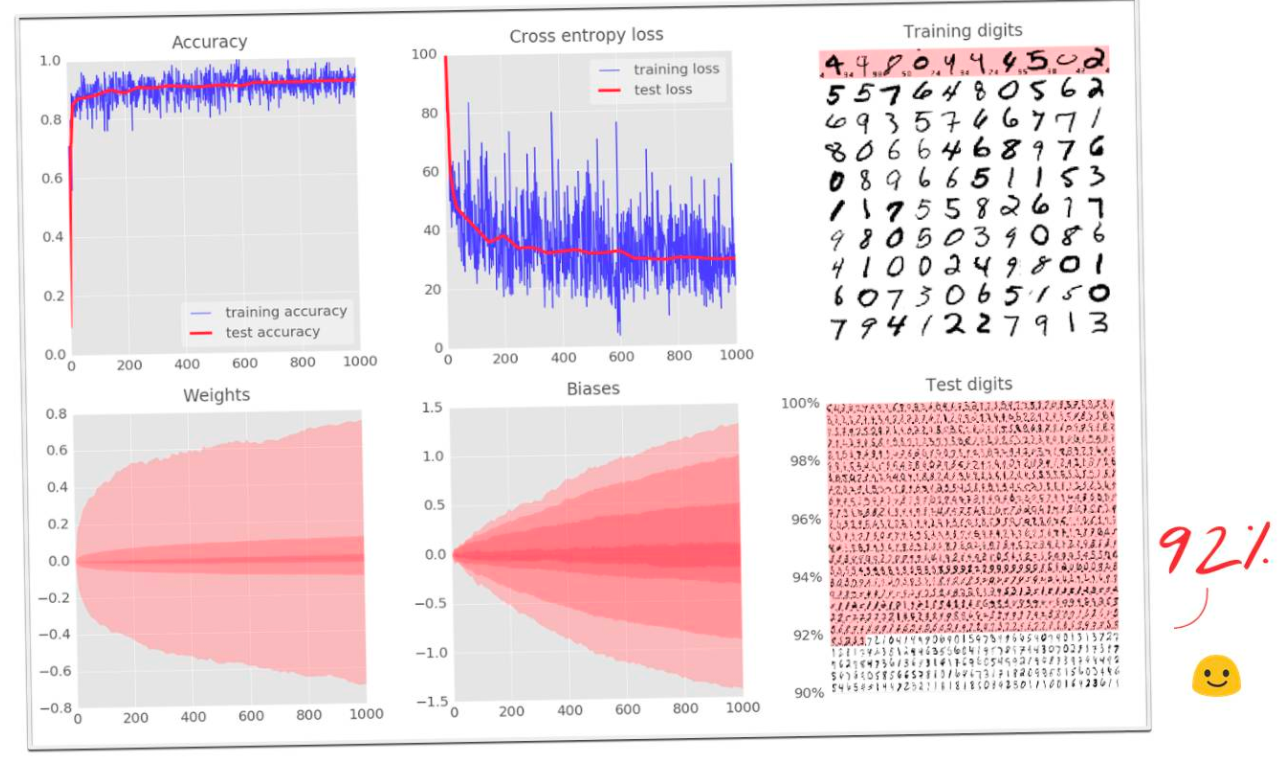
\includegraphics[width=0.8\textwidth]{figures/mnist-slp-accuracy.png}
\caption{可视化:单层感知器,运行1000次step}
 \label{fig:mnist-slp-accuracy}
\end{figure}

\end{content}